\documentclass{beamer}

\usepackage[]{mathtext}
\usepackage[T2A, TS1]{fontenc}
\usepackage[utf8]{inputenc}
\usepackage[english, russian, serbianc]{babel}

\usepackage{amsmath}
\usepackage{physics}
\usepackage[]{mathtext}
\usepackage{textpos}
\usepackage{tikz}
\usepackage[siunitx]{circuitikz}
\usetikzlibrary{calc, shapes, shapes.misc, arrows.meta, curvilinear}

\usepackage{pgfplots}
\usepgfplotslibrary{smithchart}
\pgfplotsset{compat=newest}

\tikzset{onslide/.code args={<#1>#2}{%
  \only<#1>{\pgfkeysalso{#2}} % \pgfkeysalso doesn't change the path
}}

\usetheme{Boadilla}
\usecolortheme{seahorse}

\setbeamertemplate{title page}[default][colsep=-4bp,rounded=true]



\AtBeginSection[]
{
  \begin{frame}
    \frametitle{Садржај}
    \tableofcontents[currentsection]
  \end{frame}
}

\title[Асиметрични рез... – преглед тезе]
{Асиметрични резонатори као елементи јединичних ћелија једнодимензионалних метаматеријала}
\subtitle{Садржај и кратак опис дисертације}
\author{Војислав Милошевић}
\institute[]{
  %\inst{1}%
  Институт за физику Београд
}

\begin{document}

\begin{frame}

\maketitle

\begin{tikzpicture}[remember picture,overlay]
\node[anchor=east, yshift=-0.7cm, xshift=-0.2cm] at (current page.east) {\includegraphics[height=2.2cm]{logo-IPB-black.eps}};
%\node[anchor=west, yshift=-0.7cm, xshift=0.3cm] at (current page.west) {\includegraphics[height=2.5cm]{University_of_Hawaii_seal.png}};
\end{tikzpicture}

\end{frame}

\addtobeamertemplate{frametitle}{}{%
\begin{textblock*}{100mm}(.93\textwidth,-0.95cm)
\includegraphics[height=0.9cm]{logo-IPB-black.eps}~%
%\includegraphics[height=0.9cm]{University_of_Hawaii_seal.png}
\end{textblock*}}

\begin{frame}
\frametitle{Садржај презентације}
\tableofcontents
\end{frame}

\section{Увод}

\begin{frame}[t]{Метаматеријали}

   \begin{columns}[c]
   \column{.5\textwidth}
   \begin{itemize}
       \item Метаматеријали
           \begin{itemize}
               \item вештачке композитне структуре
               \item обично периодичне, резонатори $<\lambda$
               \item ефективно хомогене (?)
           \end{itemize}
       \item Средина са негативним параметрима $\varepsilon$ и $\mu$
           \begin{itemize}
               \item Негативна рефракција

           \item Савршено сочиво
               \item Реализација помоћу метаматеријала
           \end{itemize}
   \end{itemize}
   \column{.5\textwidth}
   \centering
   \begin{tikzpicture}[scale=0.5]
        \draw[fill=lightgray] (-4,-4) rectangle (4,0);
        \draw[dashed] (0,-4) -- (0,3);
        \draw[->, very thick] (0,0) -- (30:2cm)  node[near end, below] {$\vec{k_2}$};% -- ++(0,-5);
        \draw[->, very thick] (0,0) -- (-60:3.464cm) node[near end, below left] {$\vec{k_1}$};
        \draw[->, very thick] (120:4cm) -- (120:2cm) node[near end, below left] {$\vec{S_1}$};
        \draw[->, very thin] (120:2cm) -- (0,0);% node[near end, below left] {$\vec{k_1}$};
        \draw[->] (0,1.5) arc (90:120:1.5cm) node[midway, above] {$\vartheta_1$};
        \draw[<-, very thick] (-150:3.5cm) -- (-150:1.5cm) node[near end, below ] {$\vec{S_2}$};
        \draw[->, very thin] (-150:2cm) -- (0,0);% node[near end, below left] {$\vec{k_1}$};
        \draw[->] (0,-1.5) arc (-90:-150:1.5cm) node[midway, below] {$\vartheta_2$};
        \draw[dotted] (-60:3.464cm) -- (30:2cm);
        
    \end{tikzpicture}
    \\[0.5cm]
    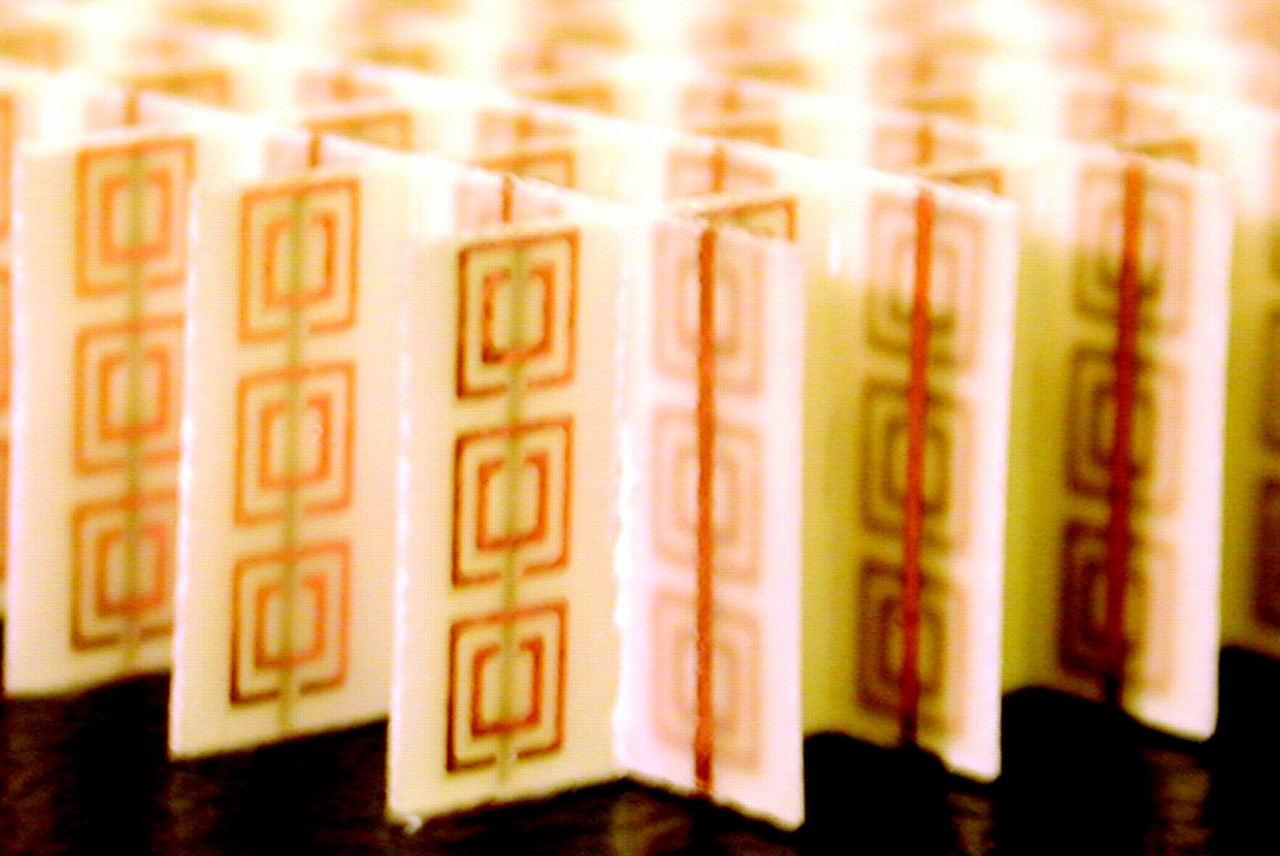
\includegraphics[width=0.7\textwidth]{sl_uvod/mm_smit.jpg}
   \end{columns} 
    
\end{frame}

\begin{frame}[t]{ММ и водови}
   \begin{columns}[c]
   \column{.5\textwidth}
   \begin{itemize}
       \item Дуални вод
\begin{align*}
    \beta l & = -\frac{\omega_c}{\omega},\\
    Z_B & = \sqrt{\frac{L}{C}} \equiv Z_C,
\end{align*}
       \item Композитни вод
       \item Резонантни приступ\\[0.5cm]
    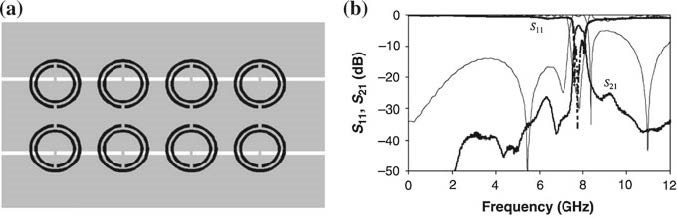
\includegraphics[width=1.0\linewidth]{sl_uvod/cpw.jpg}
   \end{itemize}
   \column{.5\textwidth}
   \begin{tikzpicture}[scale=0.8]
        \ctikzset{tripoles/mos style/arrows}
        \draw 
            (-2,0) to [short] ++(0.75,0)
            to [L=$L$] ++(2.5,0)
            to [short] ++(0.75,0)


            (-1.25,0) to [C=$C$] ++(0,-2)
            node [ground] {}

            (1.25,0) to [C=$C$]++(0,-2)
            node [ground] {}

            ;
        \draw[dashed]
            (-2,0) -- ++(-1,0)
            (2,0) -- ++(1,0)
            ;
        \draw[<->] (-1.25,1) -- (1.25,1) node[midway,above] {$l$};
        \draw[densely dashed] (-1.25,0) -- ++(0,1.2)
            (1.25,0) -- ++(0,1.2);


    \end{tikzpicture}
    \begin{tikzpicture}[scale=0.8]
        \ctikzset{tripoles/mos style/arrows}
        \draw 
            (-2,0) to [short] ++(0.75,0)
            to [C=$C$] ++(2.5,0)
            to [short] ++(0.75,0)


            (-1.25,0) to [L=$L$] ++(0,-2)
            node [ground] {}

            (1.25,0) to [L=$L$]++(0,-2)
            node [ground] {}

            ;
        \draw[dashed]
            (-2,0) -- ++(-1,0)
            (2,0) -- ++(1,0)
            ;

        \draw[dashed]
            (-2,0) -- ++(-1,0)
            (2,0) -- ++(1,0)
            ;
        \draw[<->] (-1.25,1.2) -- (1.25,1.2) node[midway,above] {$l$};
        \draw[densely dashed] (-1.25,0) -- ++(0,1.4)
            (1.25,0) -- ++(0,1.4);
    \end{tikzpicture}
   \end{columns} 
\end{frame}

\section{Екстракција параметара}

\begin{frame}[t]{Асиметричне ћелије}
    \begin{columns}[c]
        \column{.5\textwidth}

        \begin{itemize}
            \item $\varepsilon$ и $\mu$ стандардно се одређују екстракцијом параметара
            \item Метода Николсона-Роса-Вира
                \begin{itemize}
                    \item Инверзија параметара расејања
                    \item Хомогени изотропни медијум
                \end{itemize}
            \item Проблем: асиметрија (у рефлексији)
                \begin{itemize}
                    \item Могуће решење: бианизотропни медијум и одговарајућа екстракција
                    \item релације
                        \begin{equation*}\label{const}
                            \begin{split}
                                \vec{D} & = \varepsilon_0\varepsilon \vec{E} + \bar{\xi}\vec{H}\\
                                \vec{B} & = \bar{\zeta} \vec{E} + \mu_0\mu \vec{H}
                            \end{split}
                        \end{equation*}
                \end{itemize}
        \end{itemize}

        \column{.5\textwidth}

        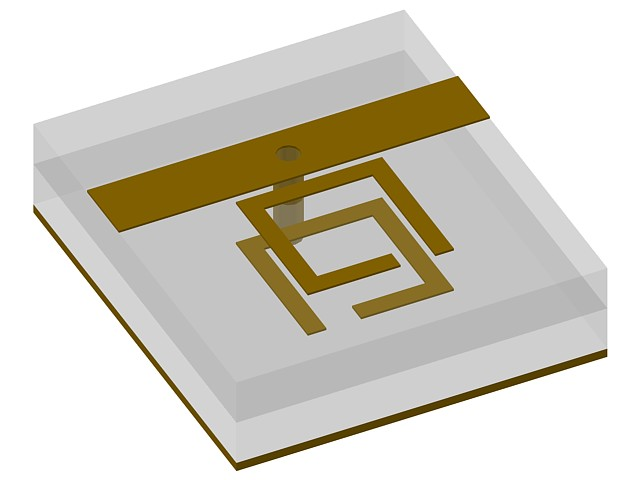
\includegraphics[width=0.75\textwidth]{slike/p2.jpeg}
        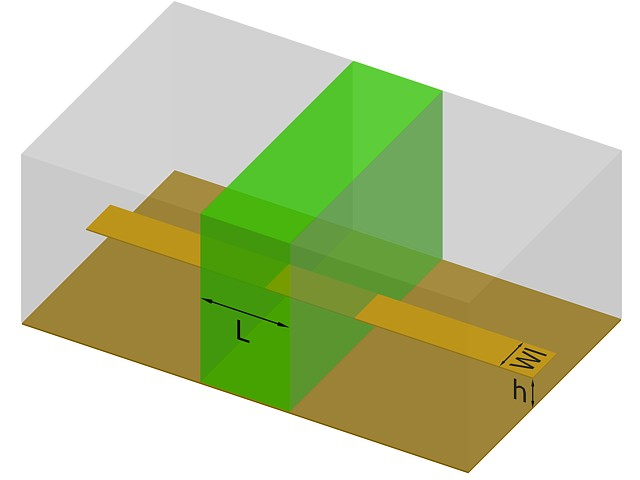
\includegraphics[width=0.8\columnwidth]{slike/slab.jpeg}

        %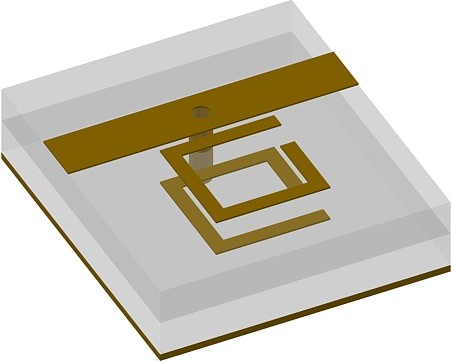
\includegraphics[width=0.75\textwidth]{slike/n1.jpeg}
    \end{columns}
\end{frame}

\begin{frame}[t]{Резултати}
\begin{columns}[c]
\column{.5\textwidth}
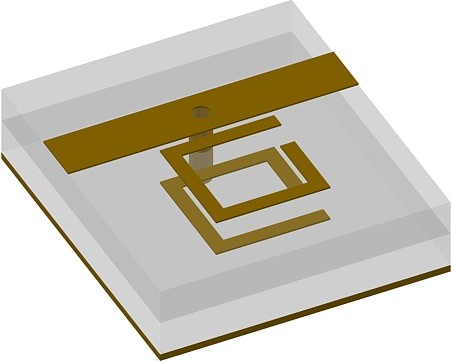
\includegraphics[width=0.65\textwidth]{slike/n1.jpeg}\\[0.5cm]
    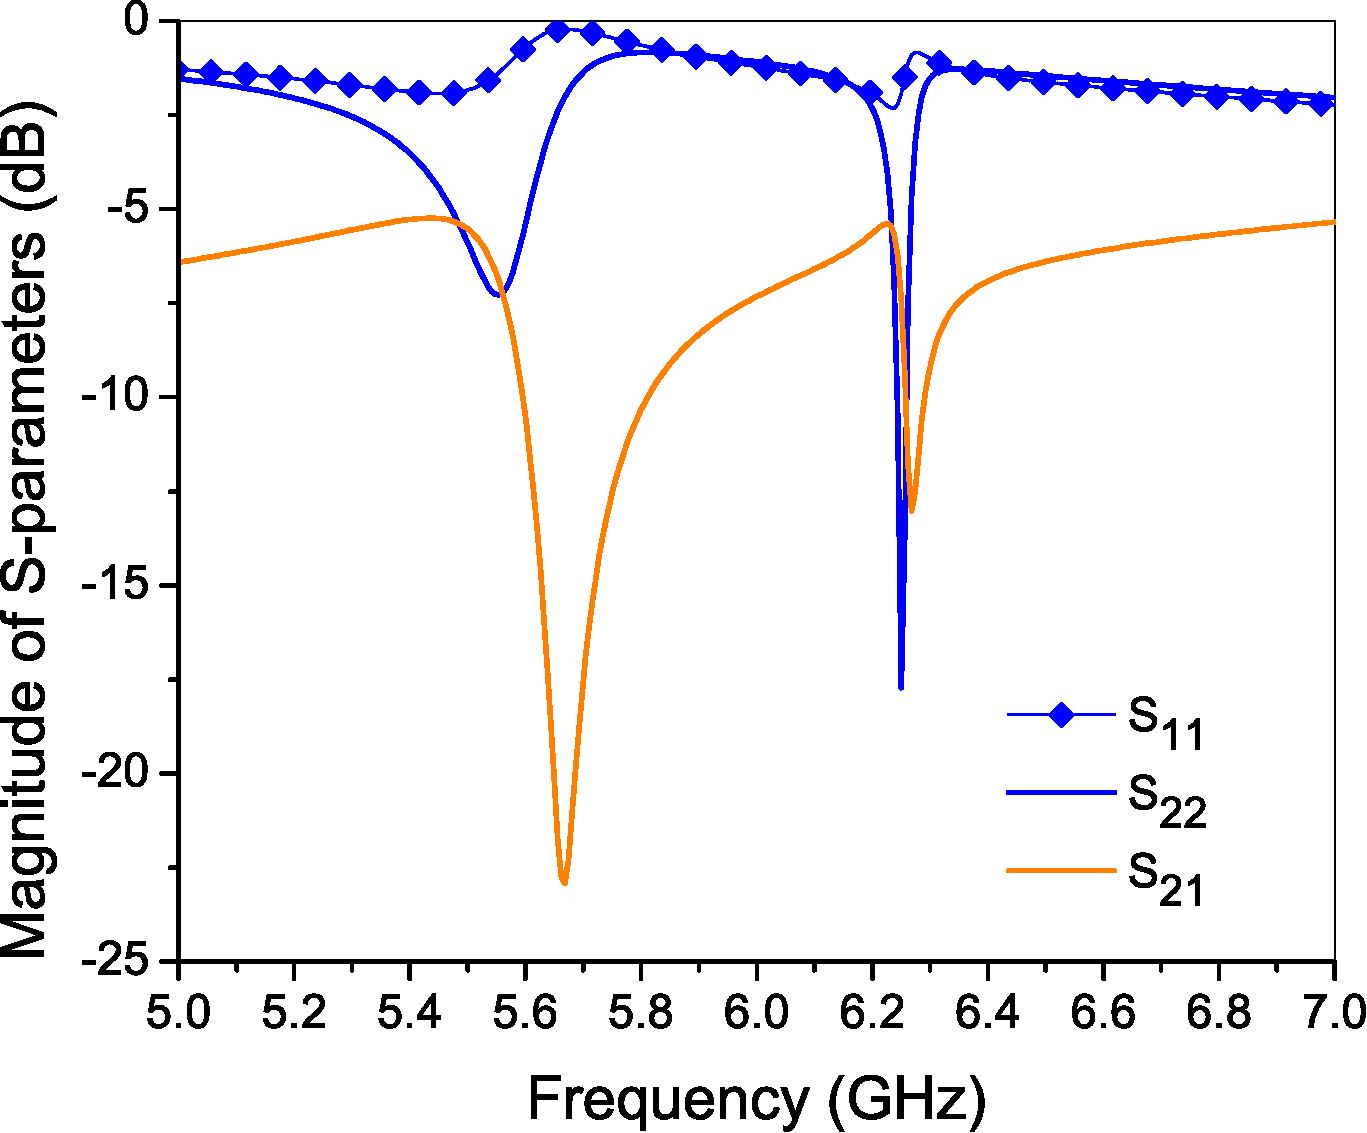
\includegraphics[width=0.70\textwidth]{slike/14a.pdf}
\column{.5\textwidth}

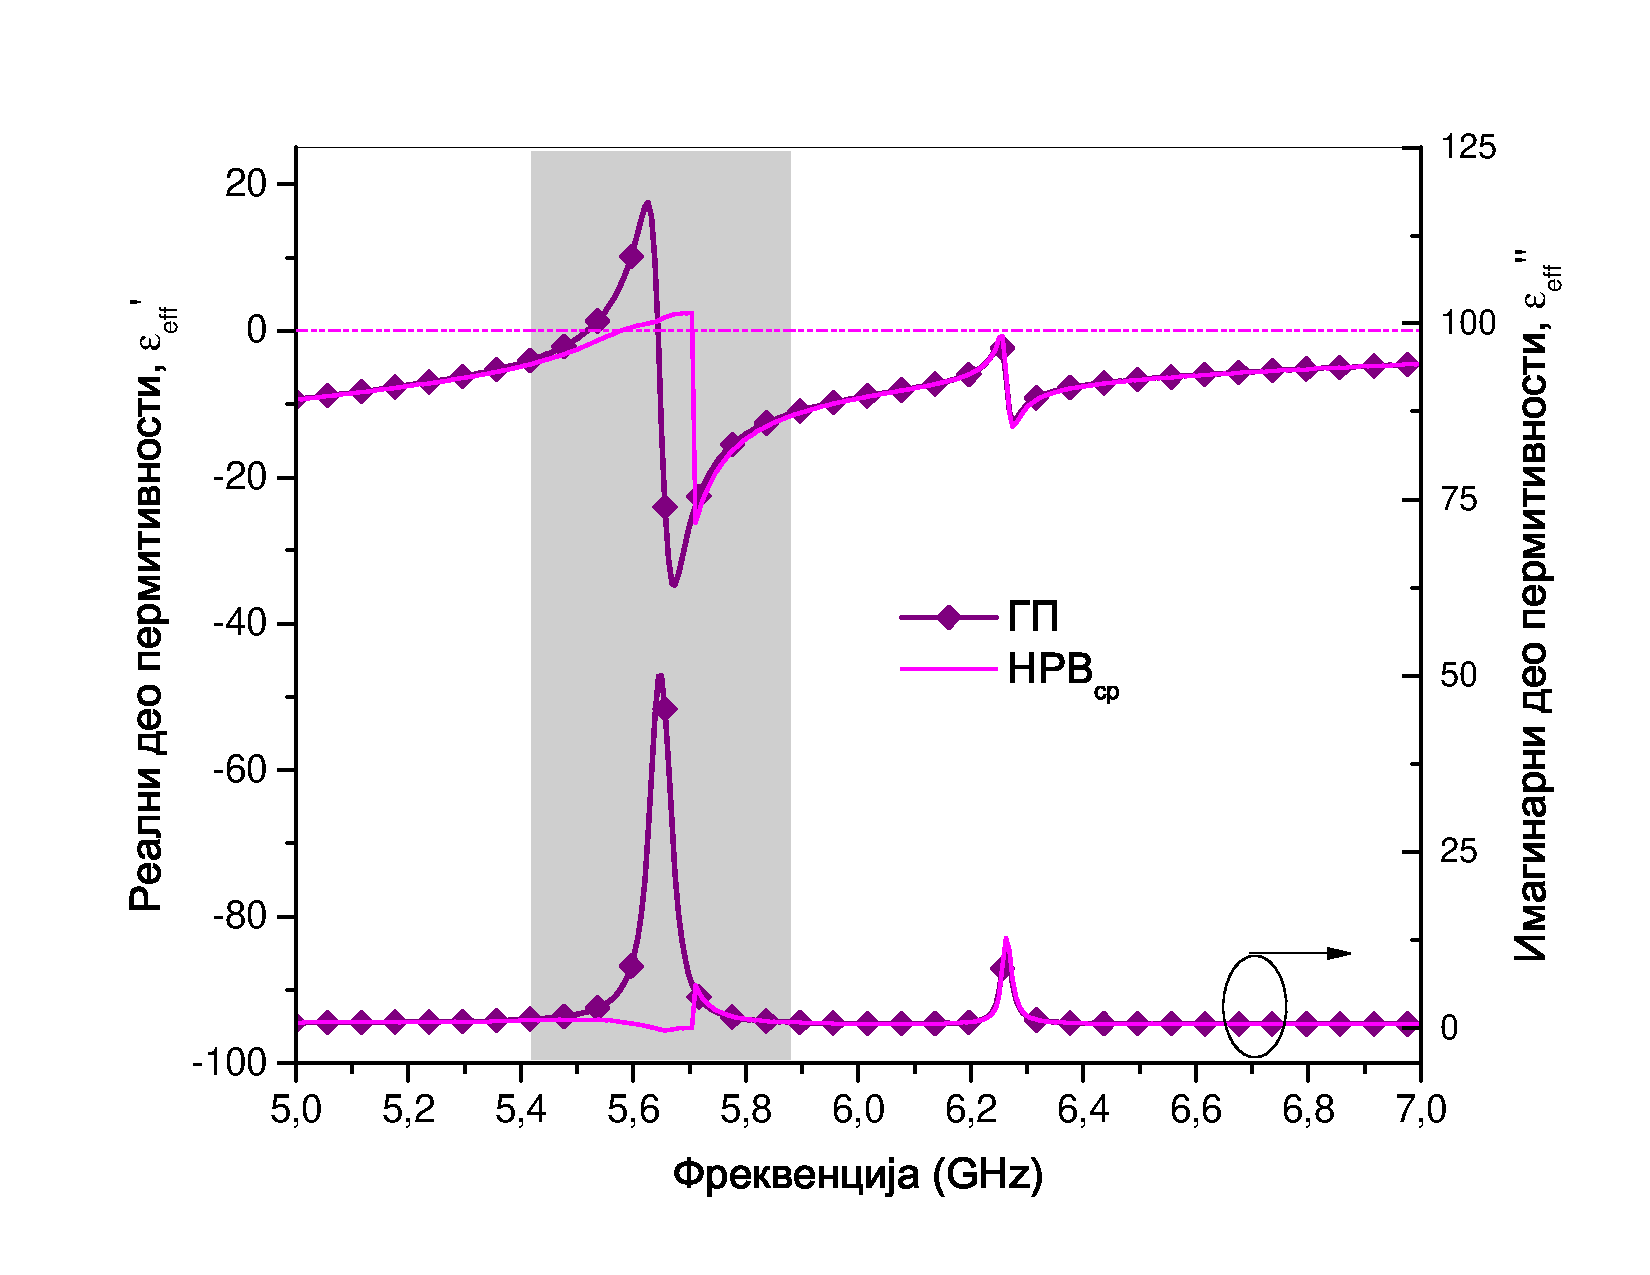
\includegraphics[width=0.85\textwidth]{slike/14c.pdf}
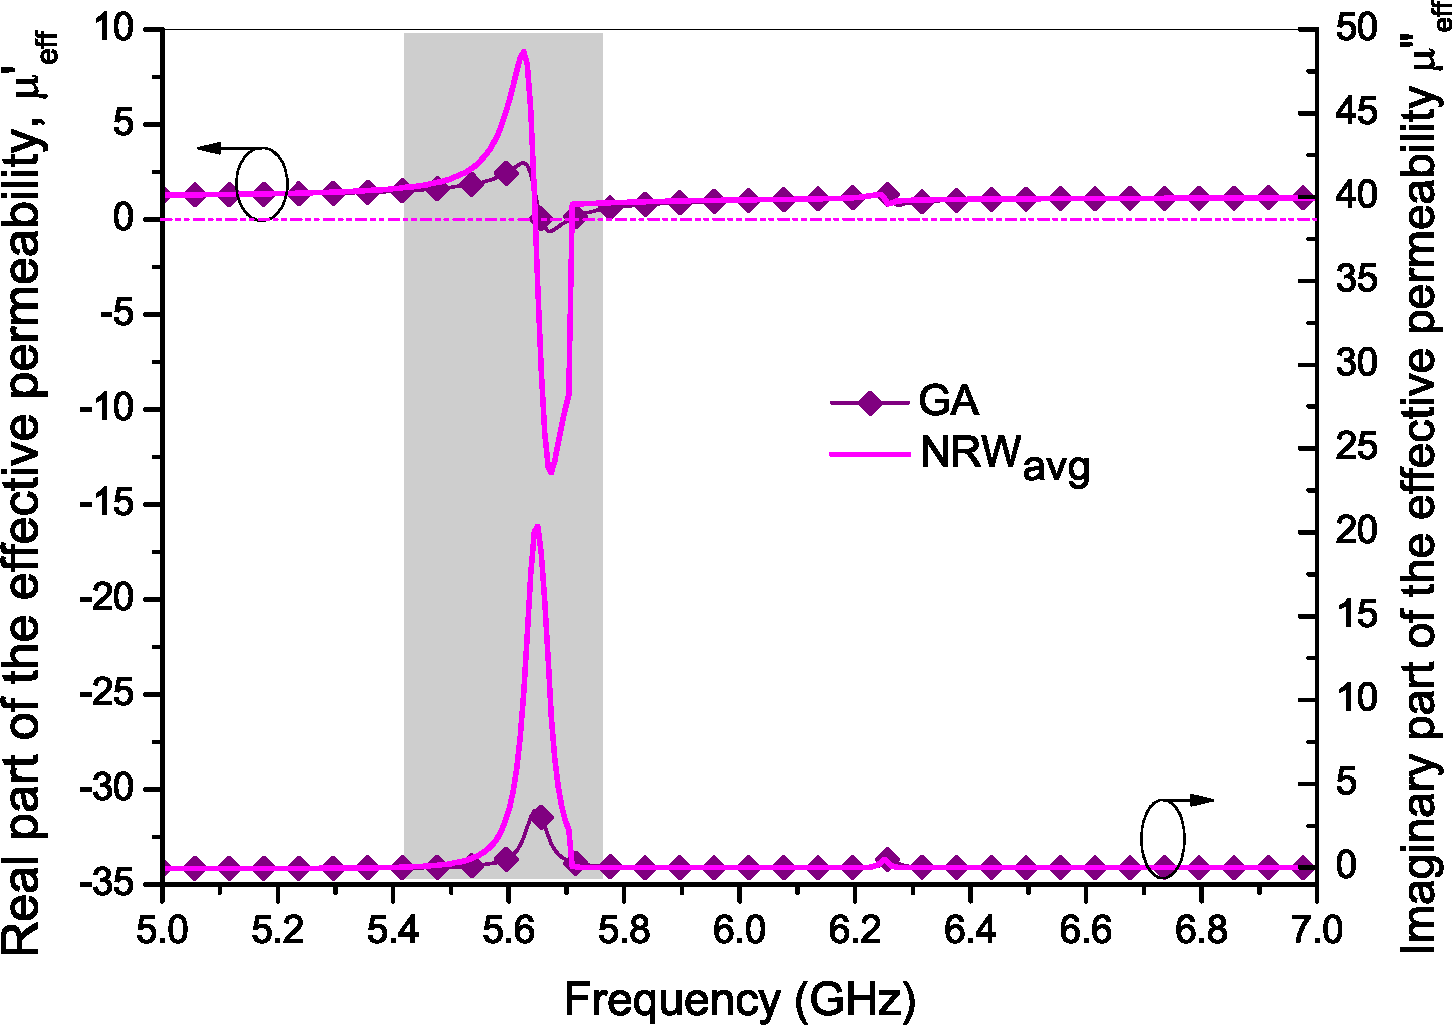
\includegraphics[width=0.85\textwidth]{slike/14e.pdf}

\end{columns}
\end{frame}

\begin{frame}[t]{Валидација}
\begin{columns}[c]
\column{.5\textwidth}
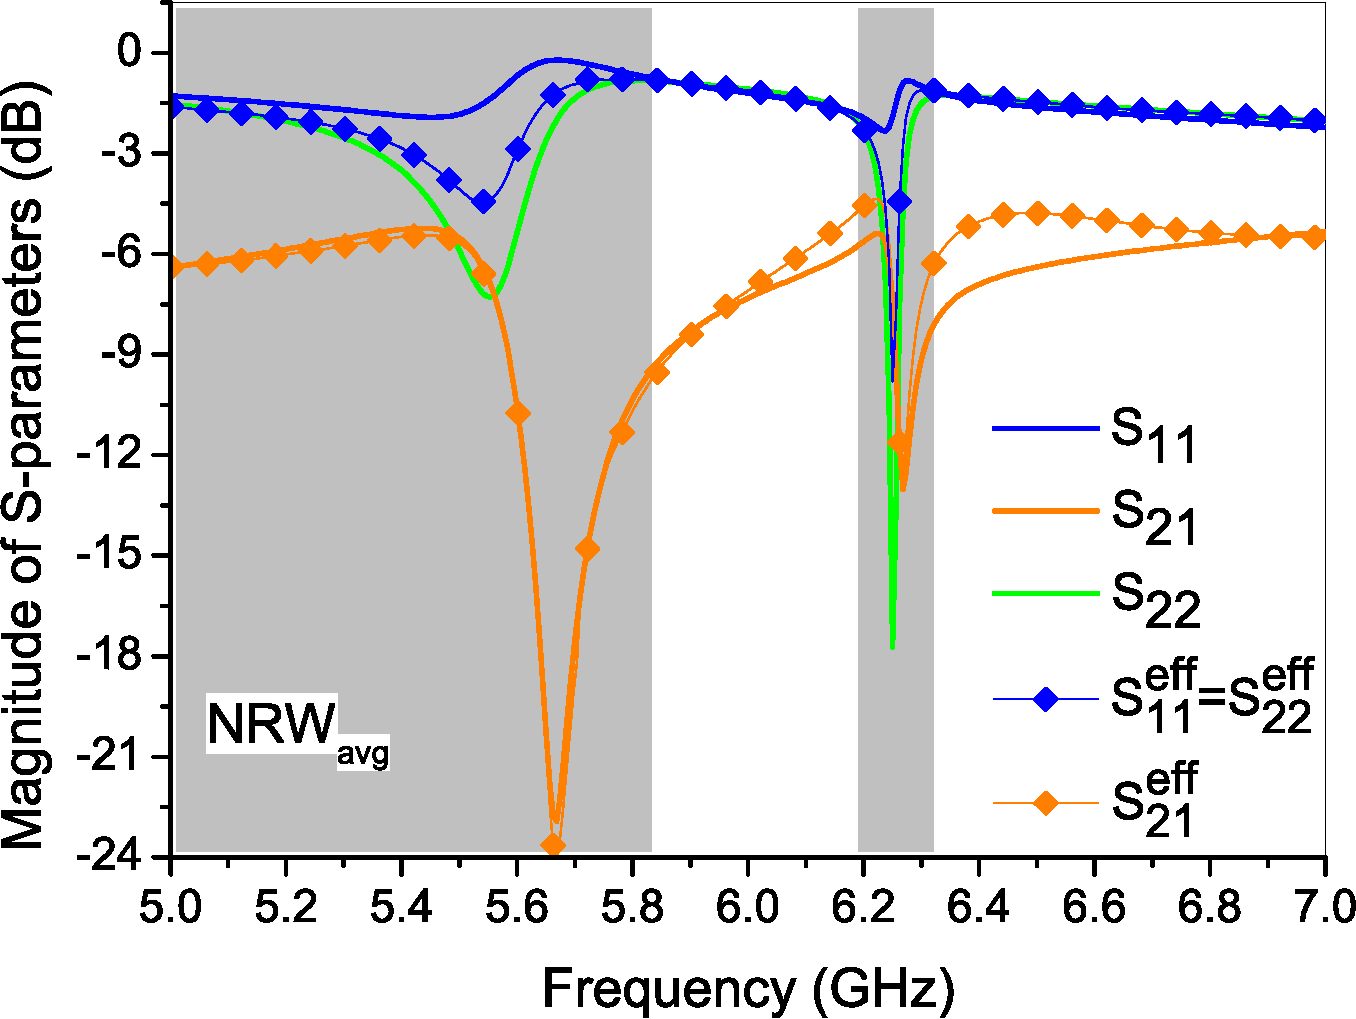
\includegraphics[width=0.80\textwidth]{slike/val90nrw_mag.pdf}
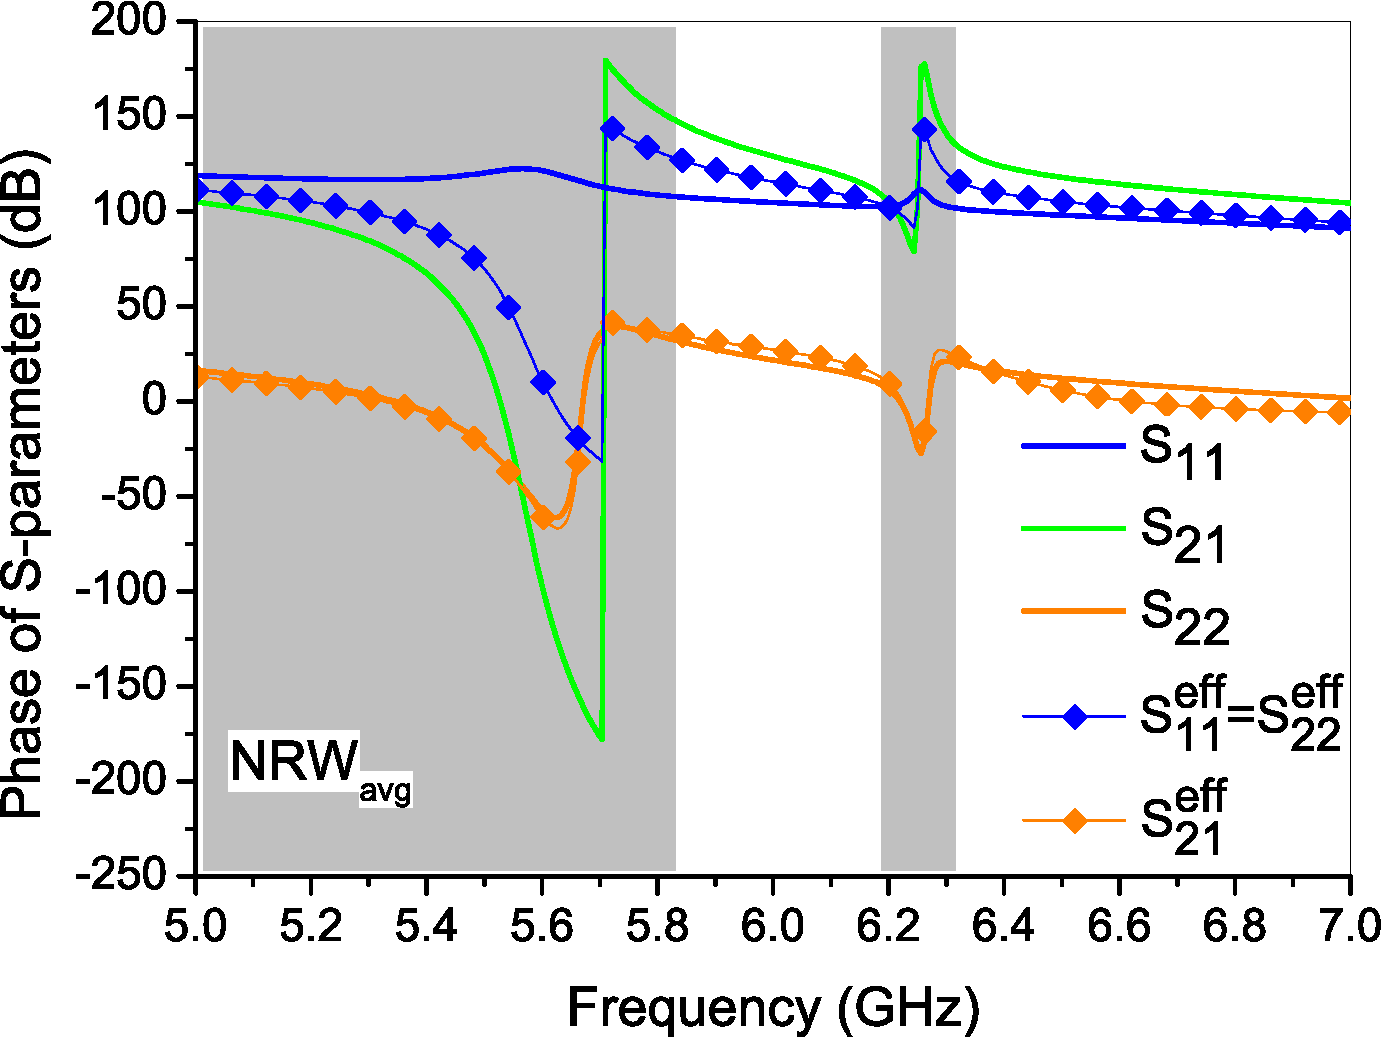
\includegraphics[width=0.80\textwidth]{slike/val90nrw_ang.pdf}

\column{.5\textwidth}

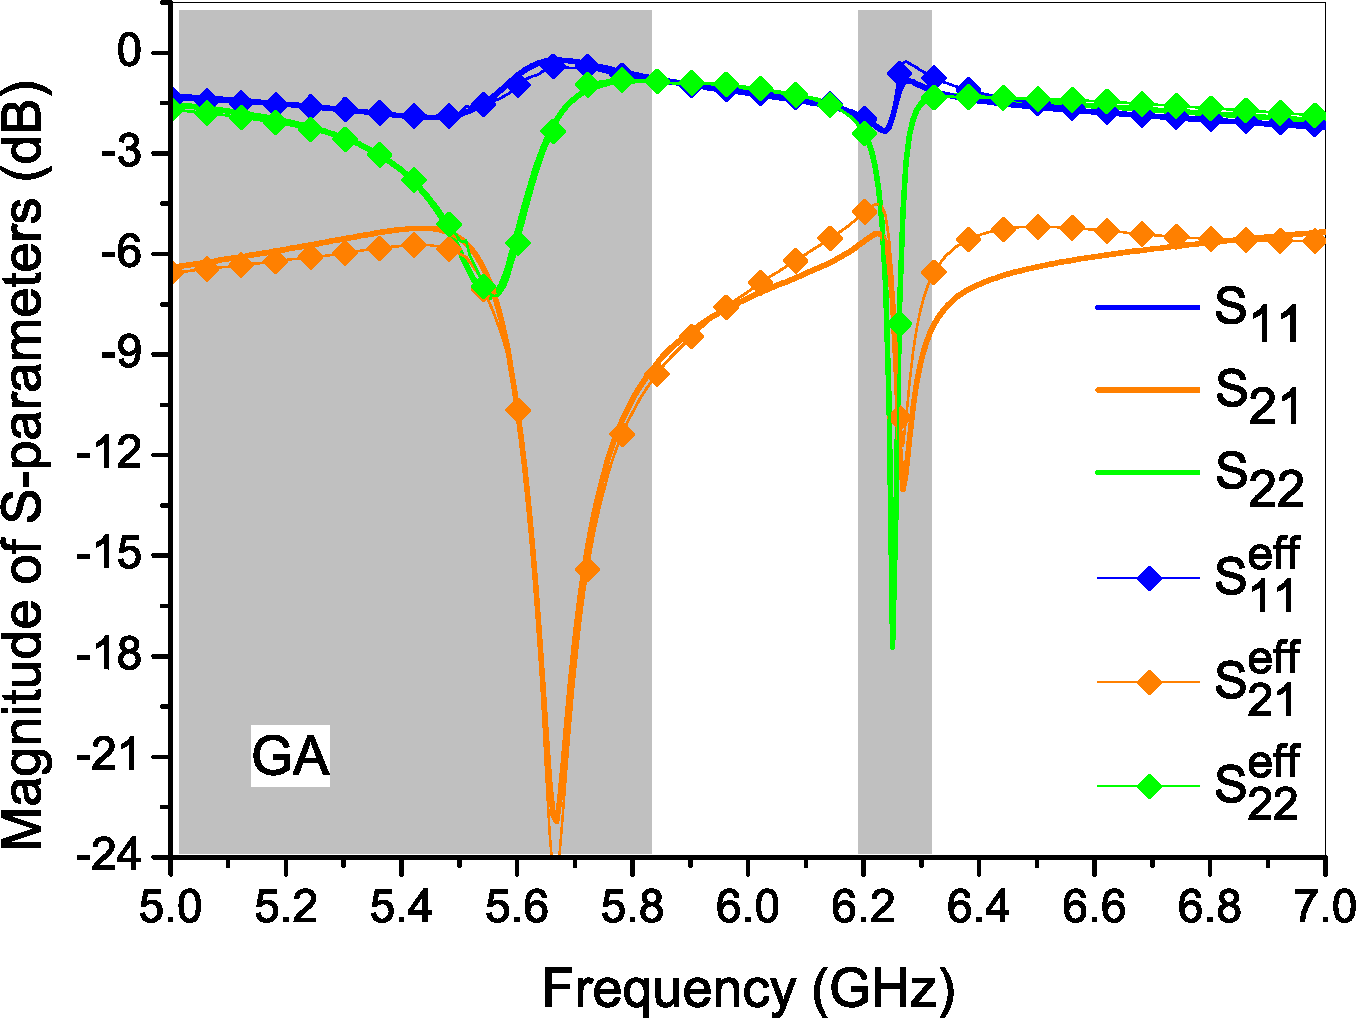
\includegraphics[width=0.80\textwidth]{slike/val90ga_mag.pdf}
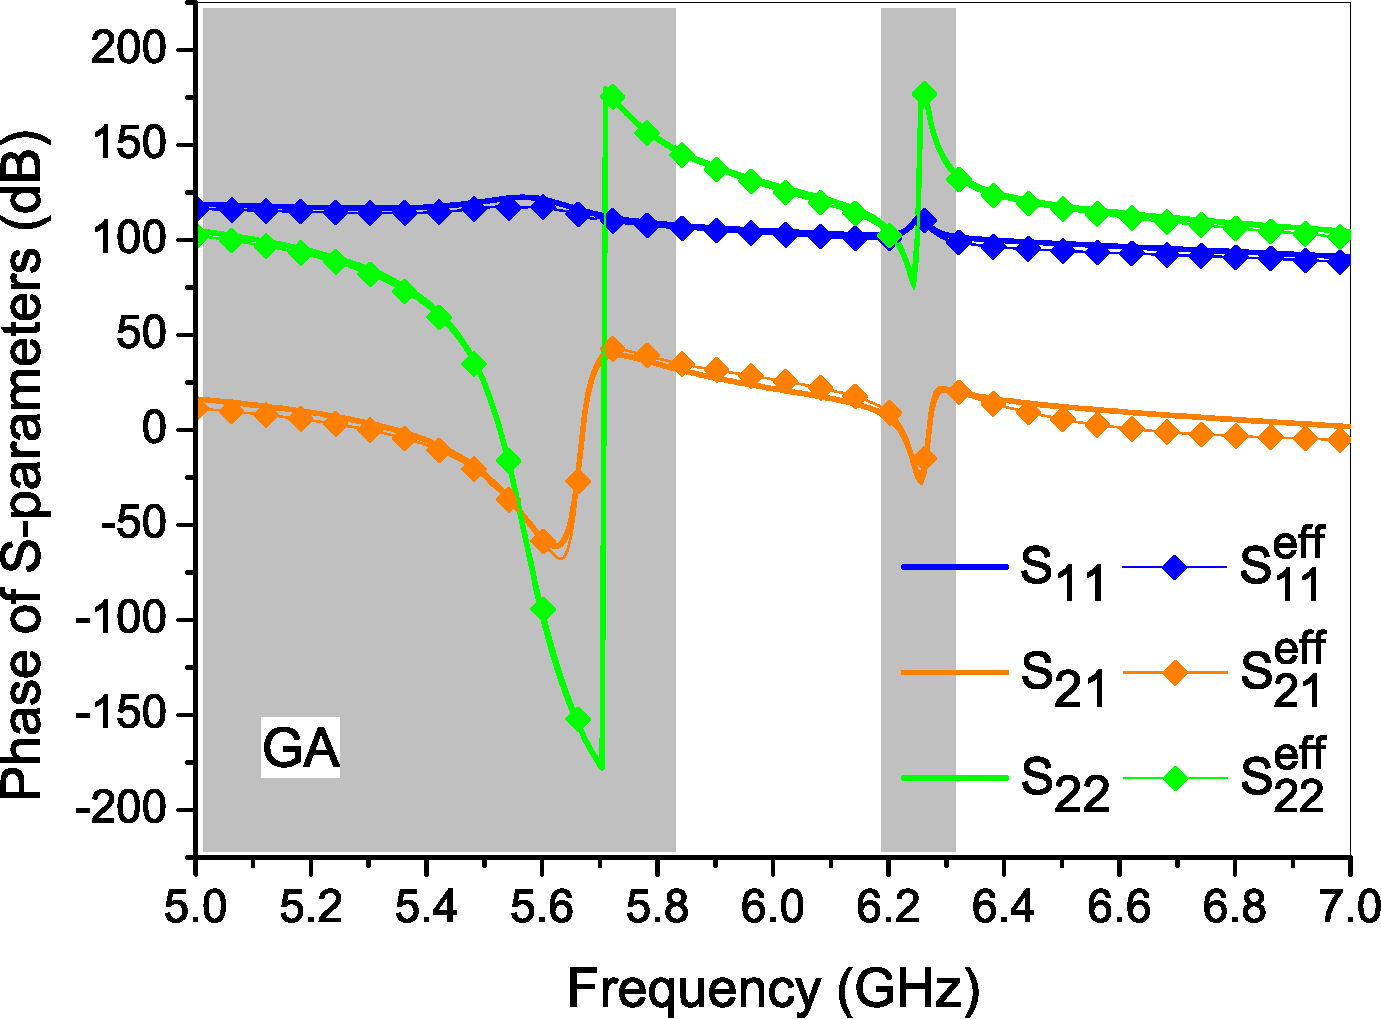
\includegraphics[width=0.80\textwidth]{slike/val90ga_ang.pdf}
\end{columns}
    
\end{frame}

\section{Еквивалентне шеме}

\begin{frame}[t]{Унапређено моделовање вода}

    \begin{columns}[c]
    \column{.5\textwidth}
    \begin{itemize}
        \item Еквивалентне шеме
            \begin{itemize}
                \item Стандардно за моделовање у $\mu$-таласној техници
                    \item Између осталог, и за водове „на бази ММ``
            \end{itemize}
        \item Проблем са $S_{11}$
            \begin{itemize}
                \item решење: 2 П ћелије за вод
            \end{itemize}
    \end{itemize}\\[0.75cm]
    \centering
    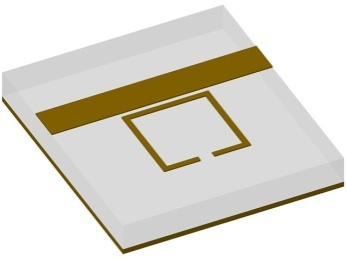
\includegraphics[width=0.7\linewidth]{sl_ekv/fig3c}
    \column{.5\textwidth}
\centering    
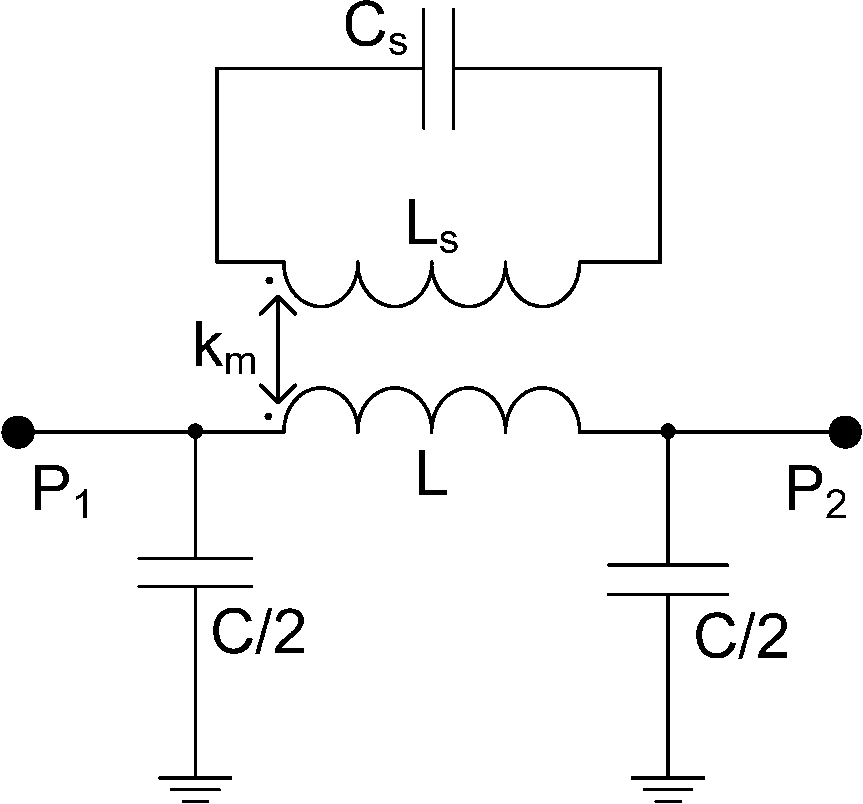
\includegraphics[scale=0.22]{sl_ekv/fig2a}\\[0.5cm]
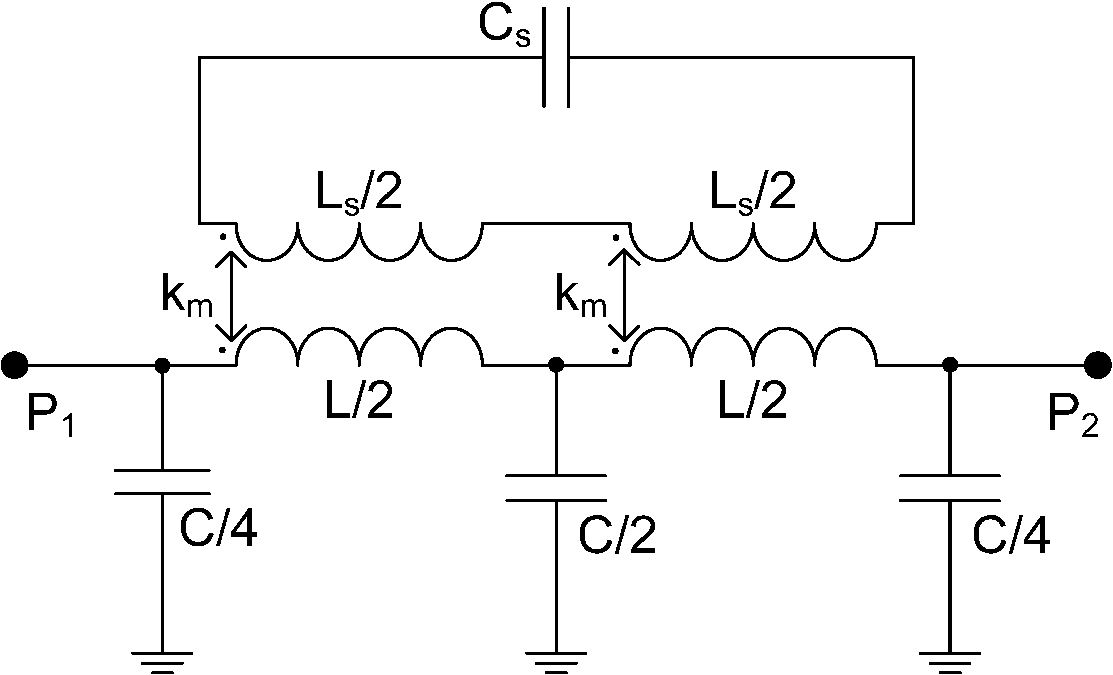
\includegraphics[scale=0.26]{sl_ekv/fig2b}
    \end{columns}
    
\end{frame}

\begin{frame}[t]{Резултати}

    \begin{columns}[c]
        \column{.5\textwidth}
        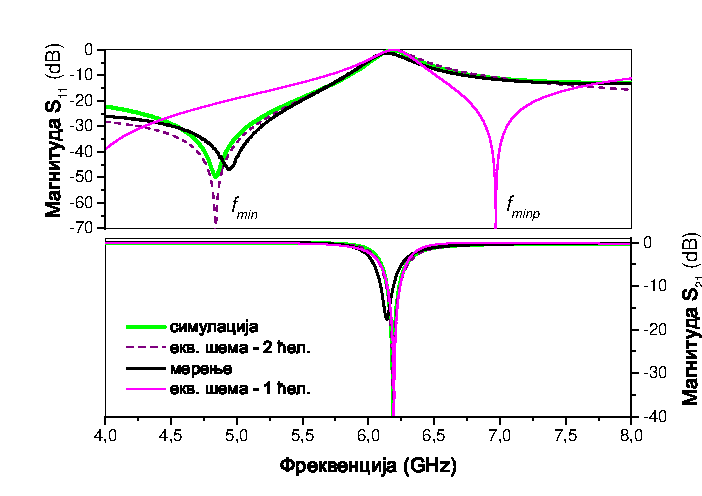
\includegraphics[width=0.85\textwidth]{sl_ekv/fig11a}
        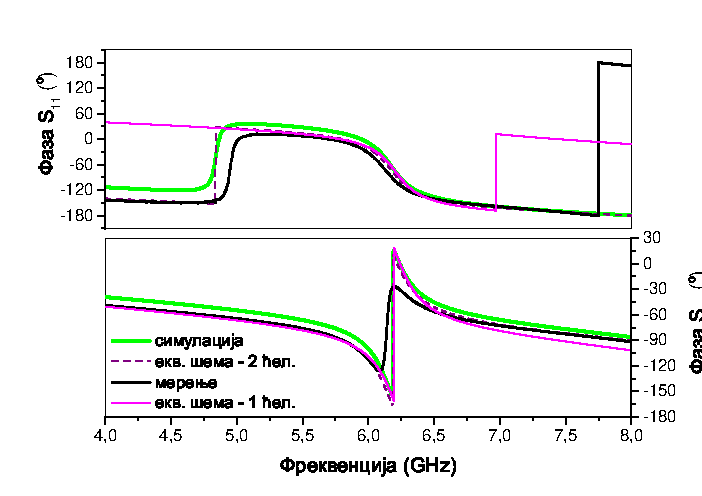
\includegraphics[width=0.85\textwidth]{sl_ekv/fig11b}

        \column{.5\textwidth}
        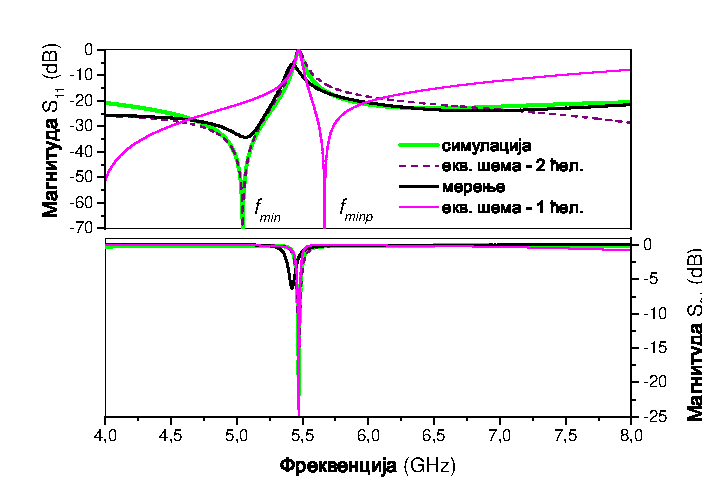
\includegraphics[width=0.85\textwidth]{sl_ekv/fig10a}
        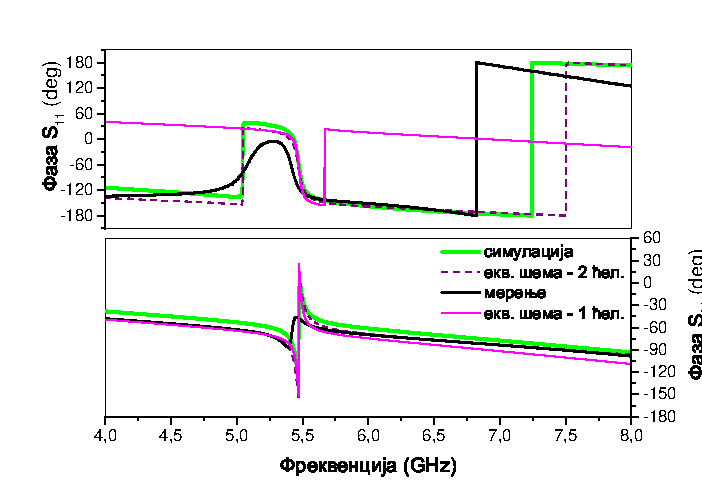
\includegraphics[width=0.85\textwidth]{sl_ekv/fig10b}

    \end{columns}
\end{frame}

\section{Класична аналогија ЕИТ-а}

\begin{frame}[t]{Електромагнетно индукована транспаренција}
    \centering
    Немогућност апсорпције у система услед кохерентне суперпозиције\\[0.5cm]
    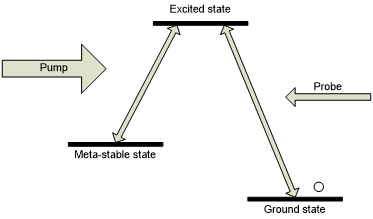
\includegraphics[width=0.5\linewidth]{sl_eit/lambda.png}
    \begin{equation*}
            H = \hbar \left\{ -\delta_p\dyad{2}{2} - \delta_c\dyad{3}{3} - \frac{1}{2}\left( \Omega_p \dyad{2}{1} + \Omega_c \dyad{3}{1}\right) + \textit{х.к.}  \right\}
        \end{equation*}
        \begin{equation*}
                \dot \rho_{21} = \frac{i}{2}\Omega_p(\rho_{11}-\rho_{22}) + \frac{i}{2}\Omega_c\rho_{32} + i\delta_p\rho_{21} - \gamma_{21}\rho_{21}
            \end{equation*}
\end{frame}

\begin{frame}[t]{Аналогија у метаматеријалима}
    \begin{equation*}
        \label{eq:pomeraj}
        x_1 = \frac{\left( \omega_0^2 - \omega^2 + j\omega\gamma_2 \right)F_0}{\kappa^2 + \left( \omega_0^2 - \omega^2 + j\omega\gamma_1 \right) \left( \omega_0^2 - \omega^2 + j\omega\gamma_2   \right)}.
    \end{equation*}\\[1cm]
    \begin{columns}[c]
    \column{.5\textwidth}
    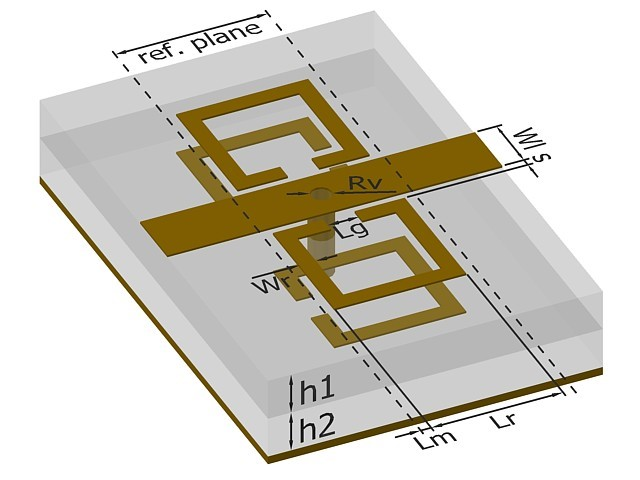
\includegraphics[width=0.8\linewidth]{sl_eit/jc2.jpg}
    \column{.5\textwidth}
    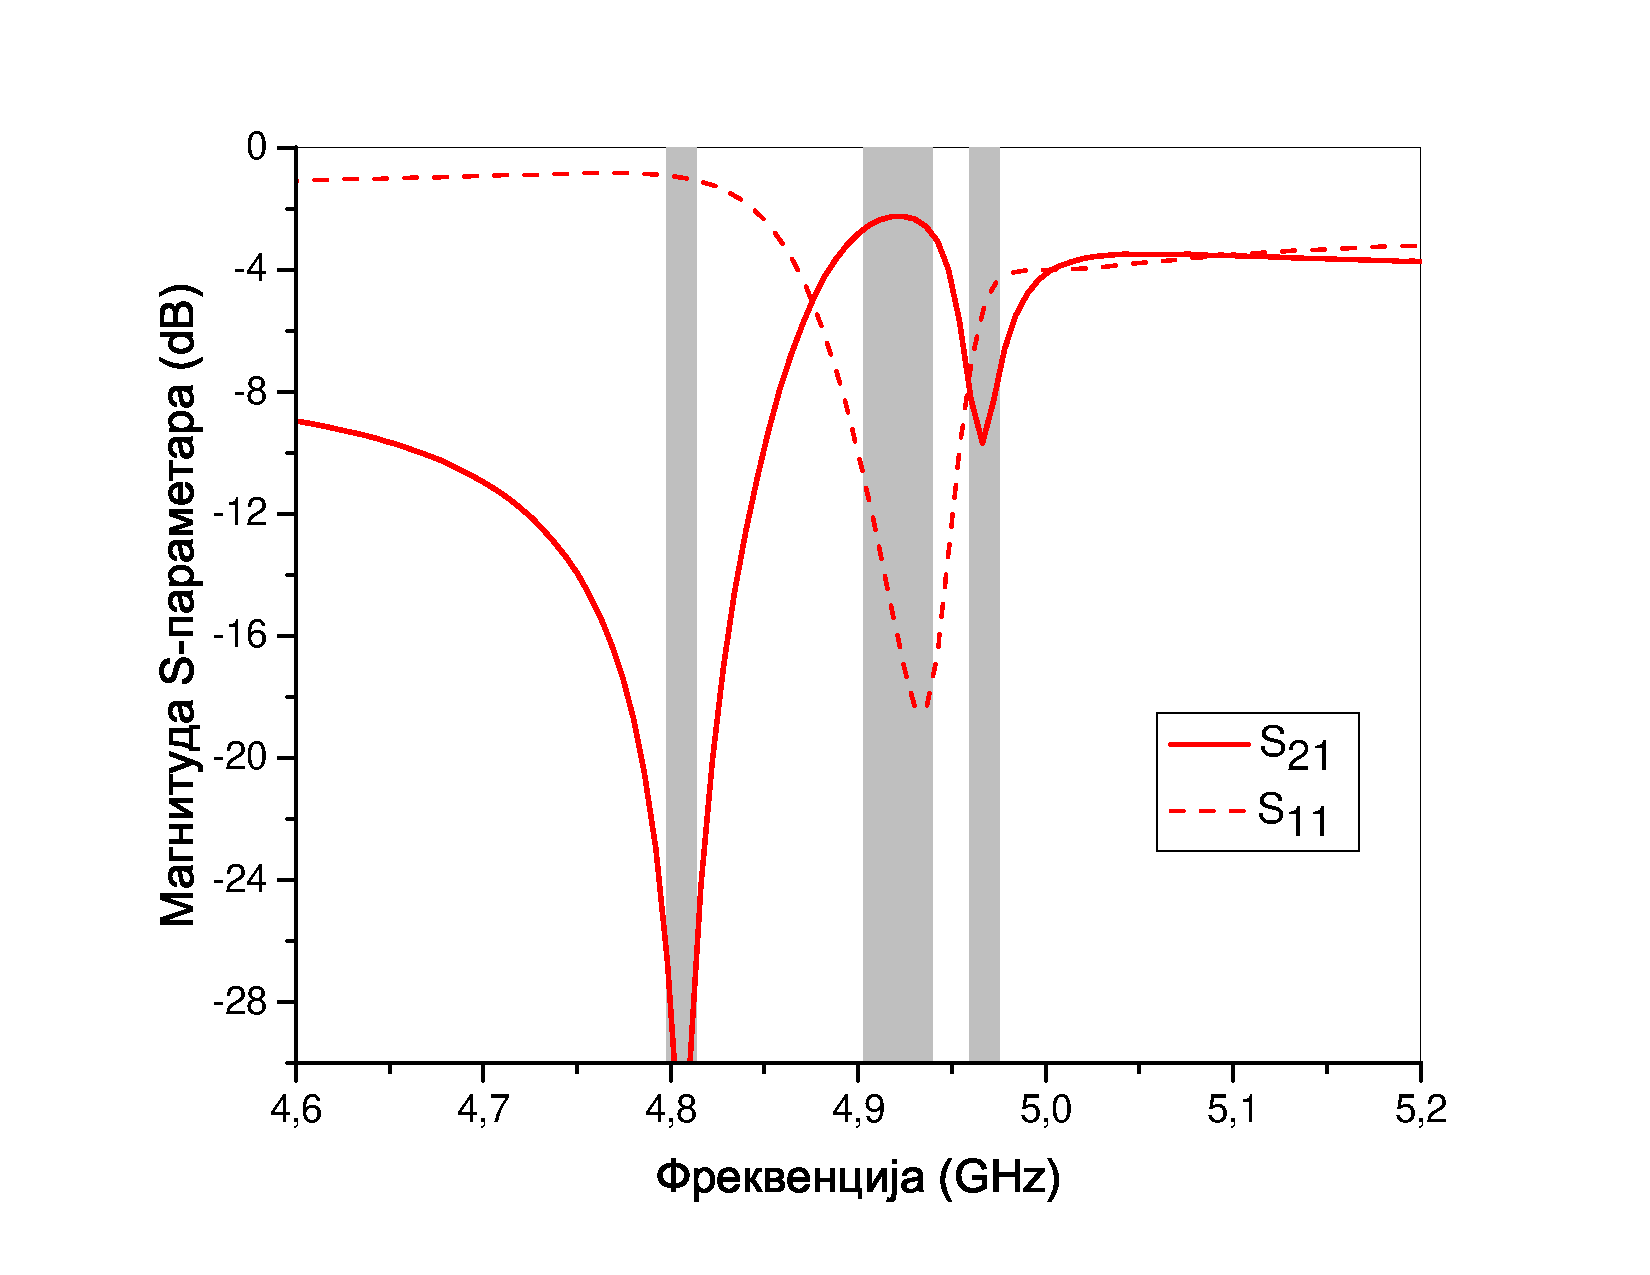
\includegraphics[width=0.8\linewidth]{sl_eit/mag.pdf}
    \end{columns}
\end{frame}

\section{Теорија спрегнутих модова}

\begin{frame}[t]{Увод}

    \begin{columns}[c]
        \column{.5\textwidth}
        \begin{itemize}
            \item Резонантно коло:
                \begin{equation*}
                    v = L \frac{d i}{d t}; \qquad i = -C \frac{d v}{d t}.
                \end{equation*}
            \item Амплитуда позитивне фреквенције: 
                \begin{equation*}
                    \alpha = \sqrt{\frac{C}{2}}\left( v + j\sqrt{\frac{L}{C}}i  \right),
                    \label{tsm:pamp}
                \end{equation*}
                \begin{equation*}
                    \frac{d\alpha}{dt} = j\omega_0 \alpha.
                    \label{tsm:smdif1}
                \end{equation*}
            \item Спрега са водом:
                \begin{equation*}
                    \frac{d\alpha}{dt} = j\omega_0 \alpha - \gamma \alpha + \kappa a,
                    \label{tsm:smdif2}
                \end{equation*}
        \end{itemize}
        \column{.5\textwidth}
        \centering    
        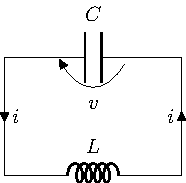
\includegraphics[width=0.6\linewidth]{sl_tsm/lckolo.pdf}\\[1cm]
        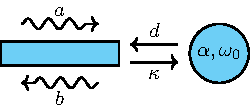
\includegraphics[width=0.8\linewidth]{sl_tsm/sm-vod1.pdf}
    \end{columns}
    
\end{frame}

\begin{frame}[t]{Примена на антисиметричне СРР-ове}
    \begin{columns}[c]
        \column{.5\textwidth}

\begin{equation*}
    \begin{split}{\scriptstyle
S_{21} = S^{(0)}_{21} + \frac{(d_1+d_2)^2}{2j(\omega-\omega_0 - \kappa) + |d_1+d_2|^2}\\
\scriptstyle- \frac{(d_1-d_2)^2}{2j(\omega-\omega_0 + \kappa) + |d_1-d_2|^2},}
\end{split}\label{tsm:cm_s21}
\end{equation*}
\begin{equation*}
\begin{split}
\scriptstyle S_{11} = S^{(0)}_{11} + \frac{(d_1+d_2)^2}{2j(\omega-\omega_0 - \kappa) + |d_1+d_2|^2}\\
\scriptstyle + \frac{(d_1-d_2)^2}{2j(\omega-\omega_0 + \kappa) + |d_1-d_2|^2}.
\end{split}\label{tsm:cm_s11}
\end{equation*}
        \column{.5\textwidth}
        \centering
        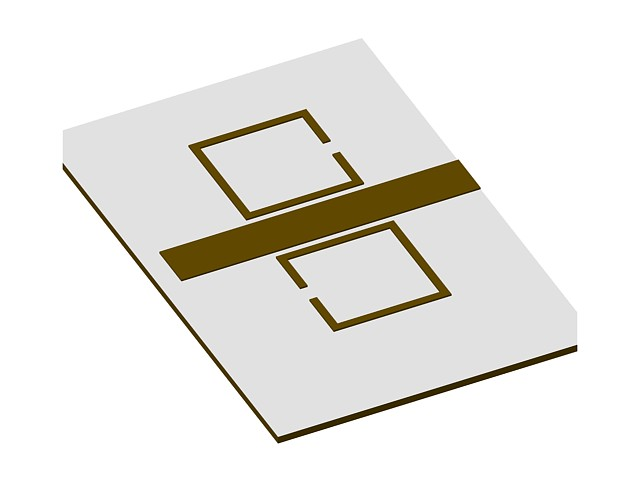
\includegraphics[width=0.7\columnwidth]{sl_tsm/pod90sr.jpeg}\\[0.5cm]
        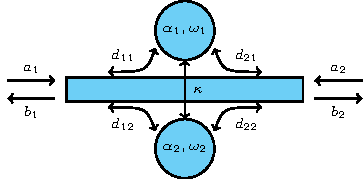
\includegraphics[scale=1]{sl_tsm/smfig.pdf}
    \end{columns}
    
\end{frame}
\begin{frame}[t]{Резултати}
   \begin{columns}[c]
   \column{.5\textwidth}
   \centering
   под \SI{0}{\degree}\\
   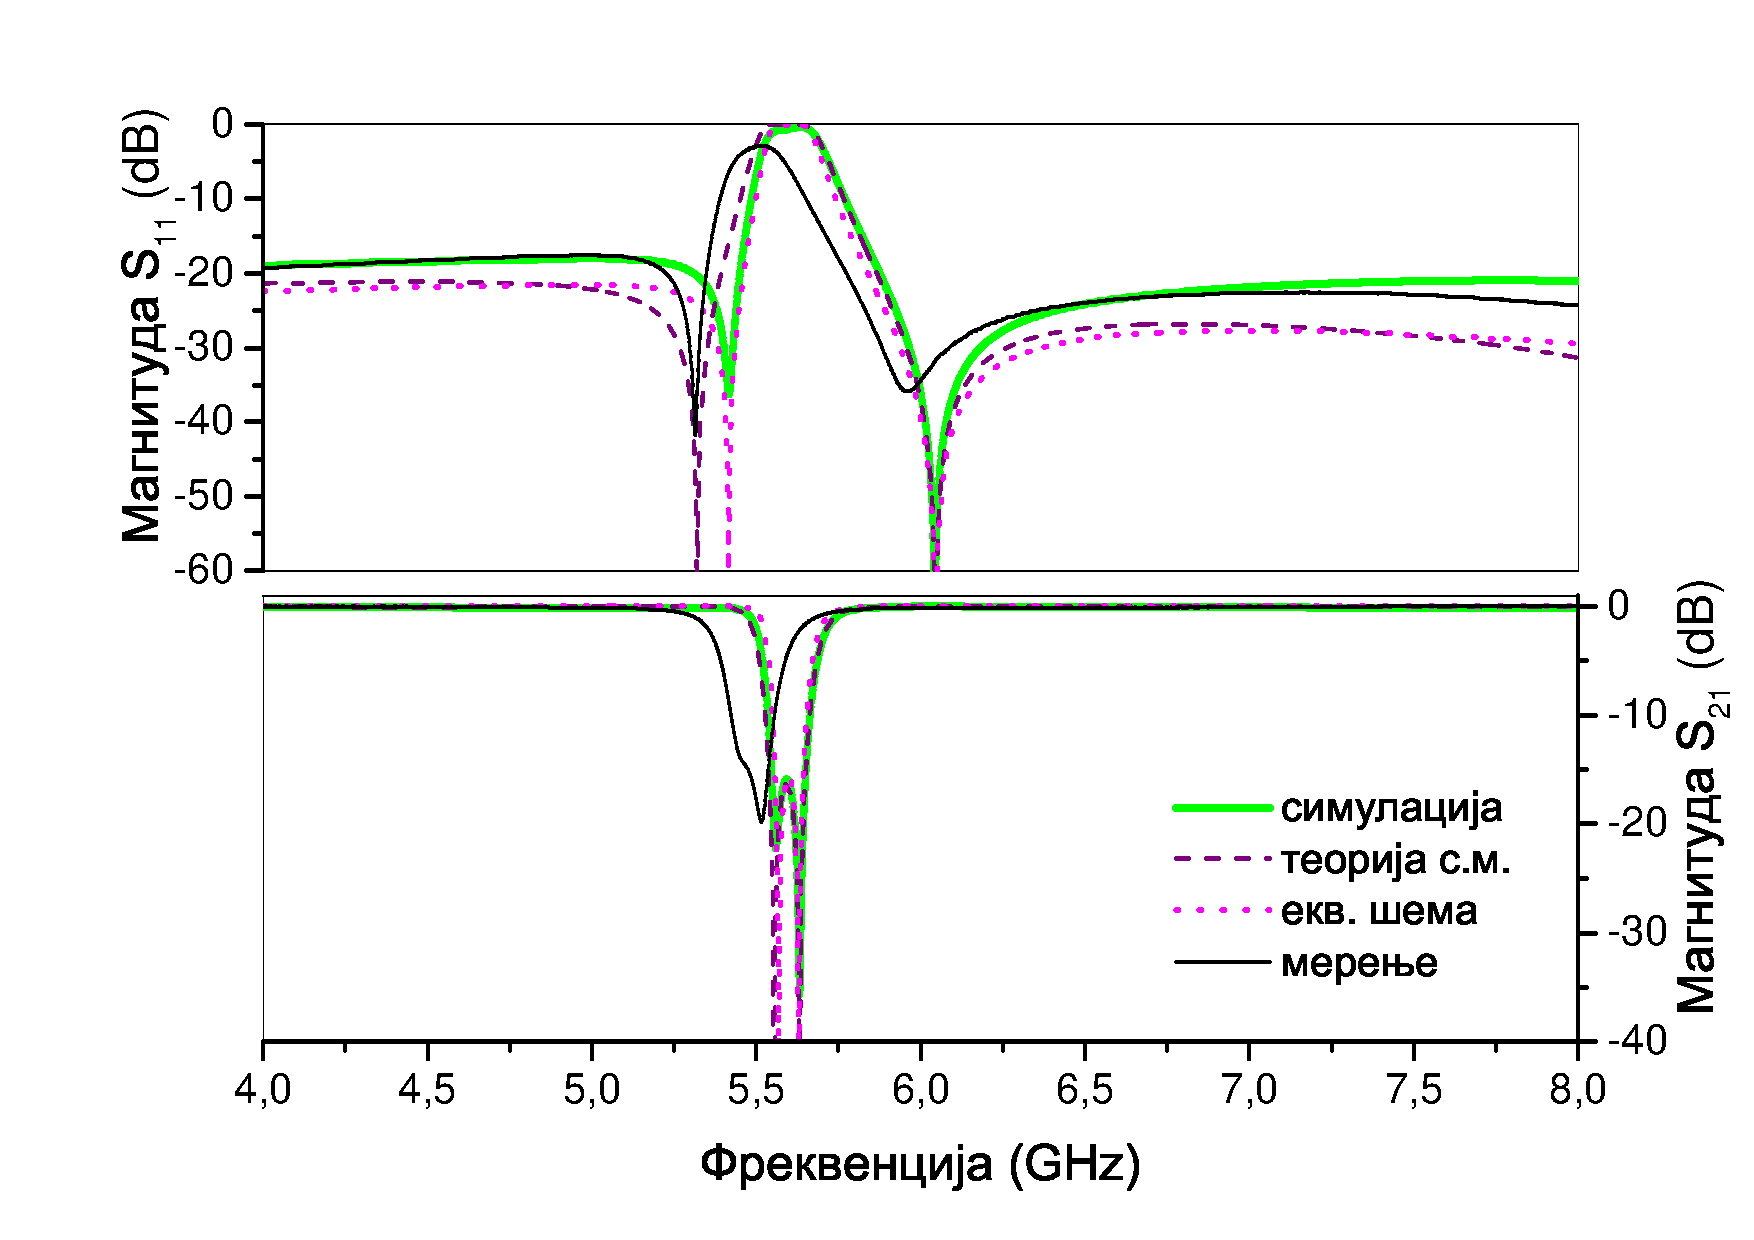
\includegraphics[width=0.8\textwidth]{sl_tsm/pod0/c_mag.pdf}\\
   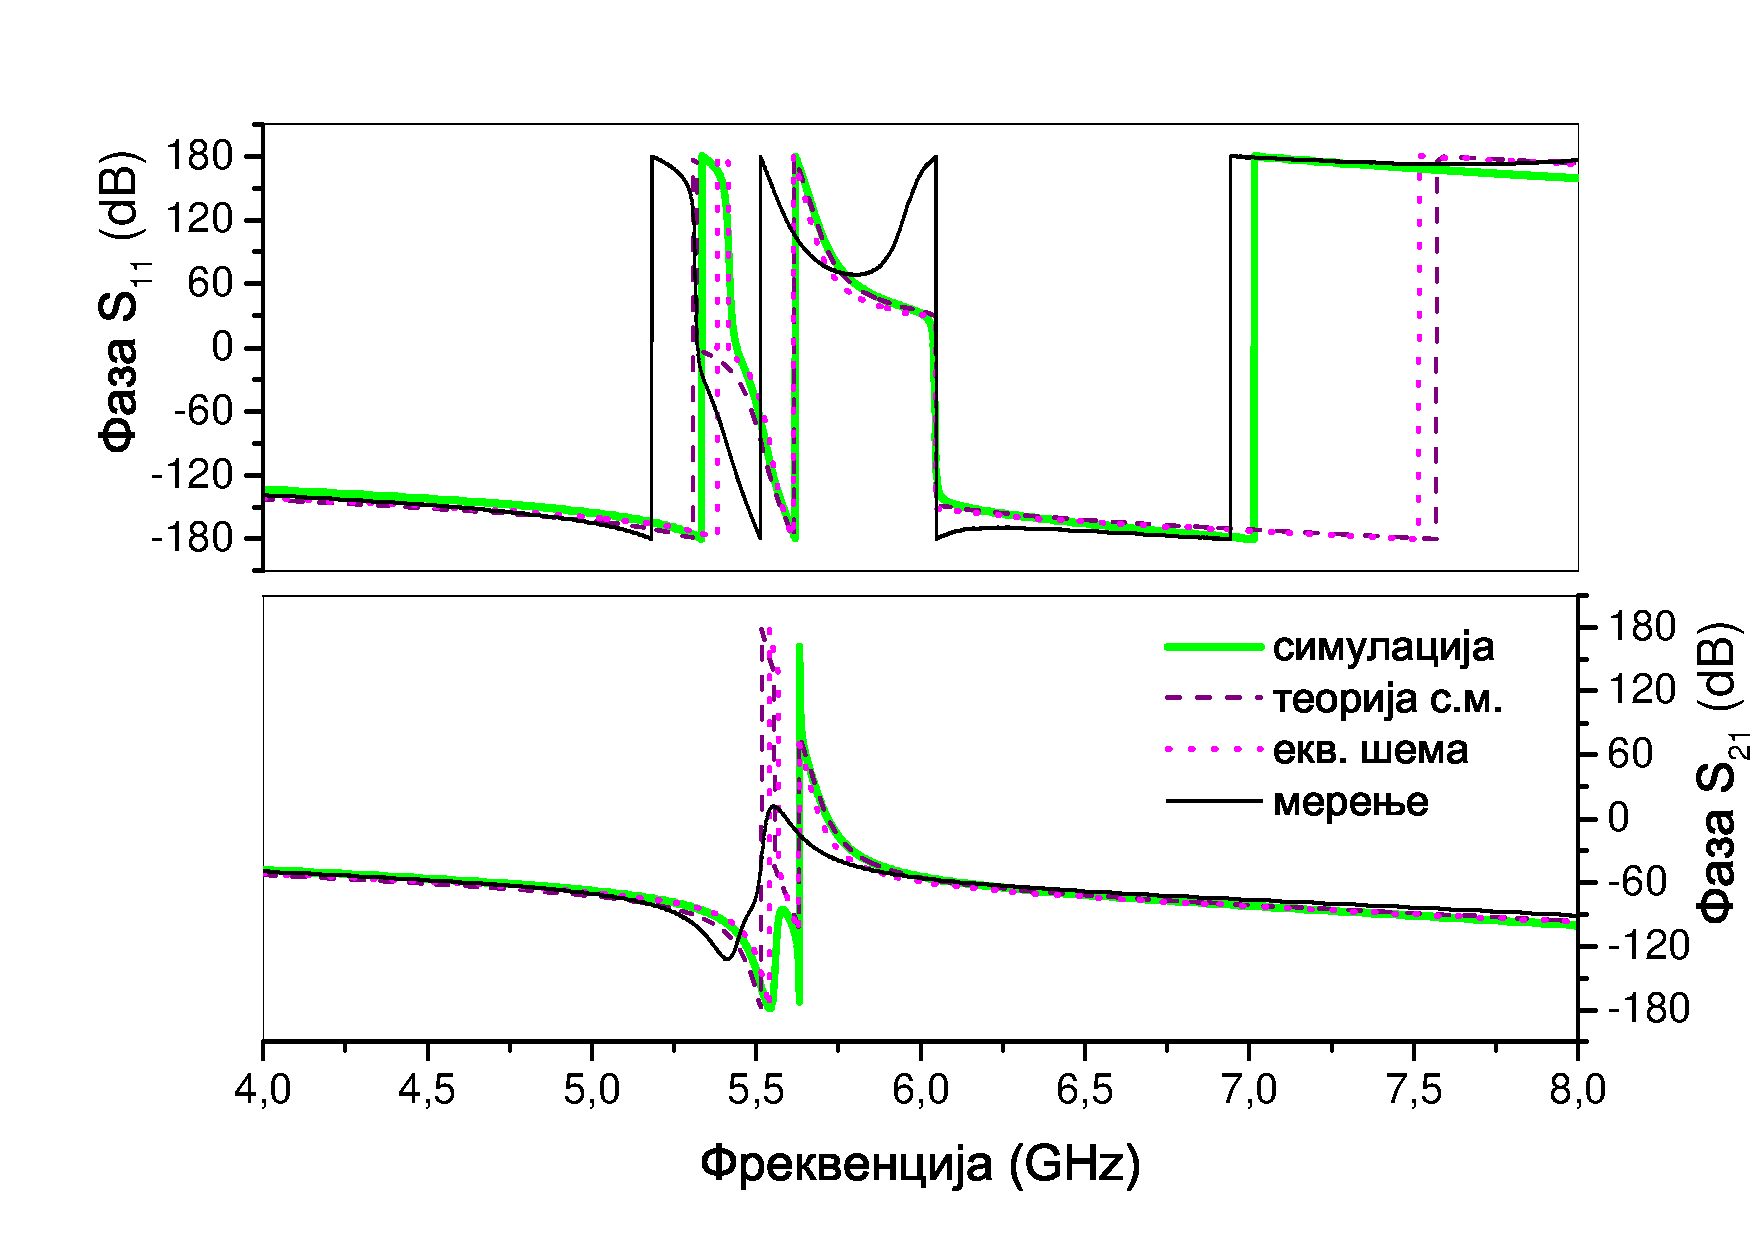
\includegraphics[width=0.8\textwidth]{sl_tsm/pod0/c_faza.pdf}\\
   \column{.5\textwidth}
   \centering
   под \SI{180}{\degree}\\
   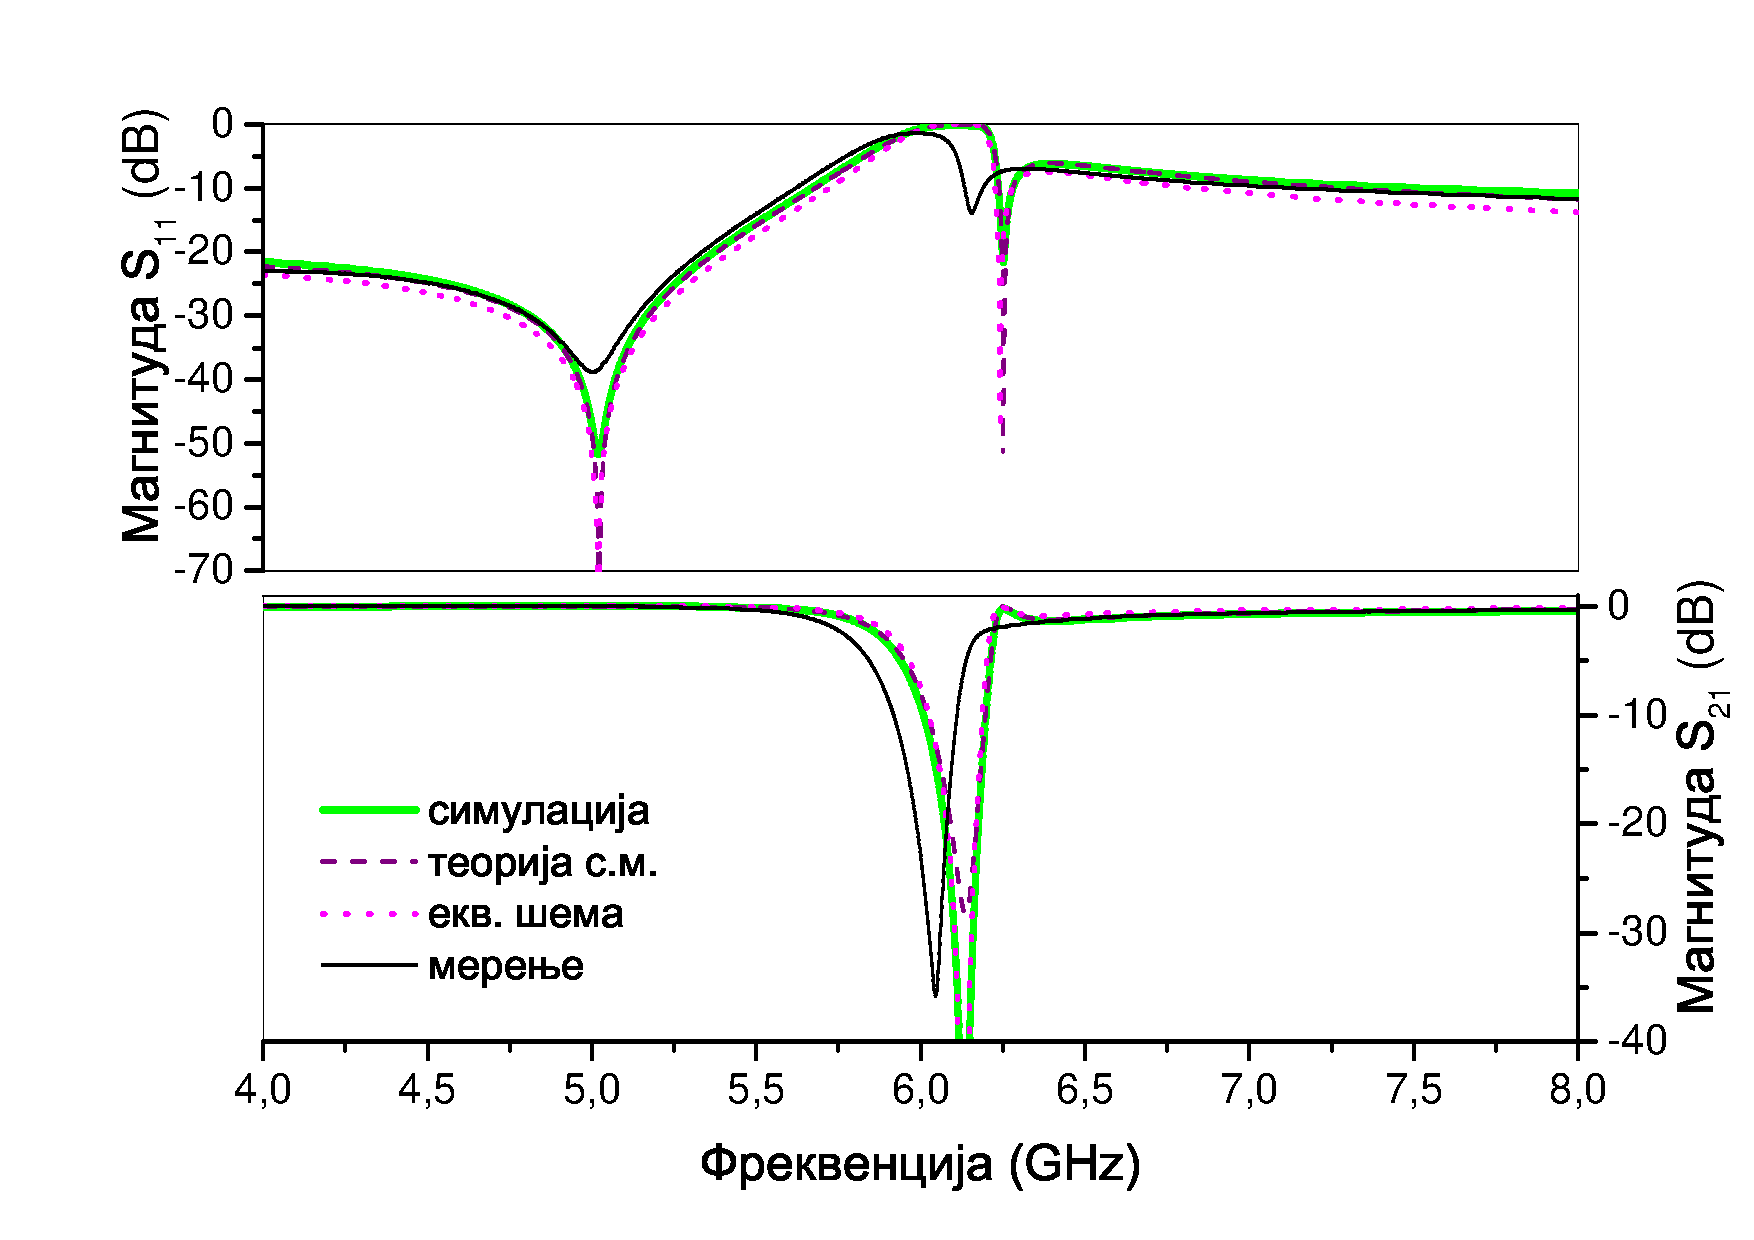
\includegraphics[width=0.8\textwidth]{sl_tsm/pod180/c_mag.pdf}\\
   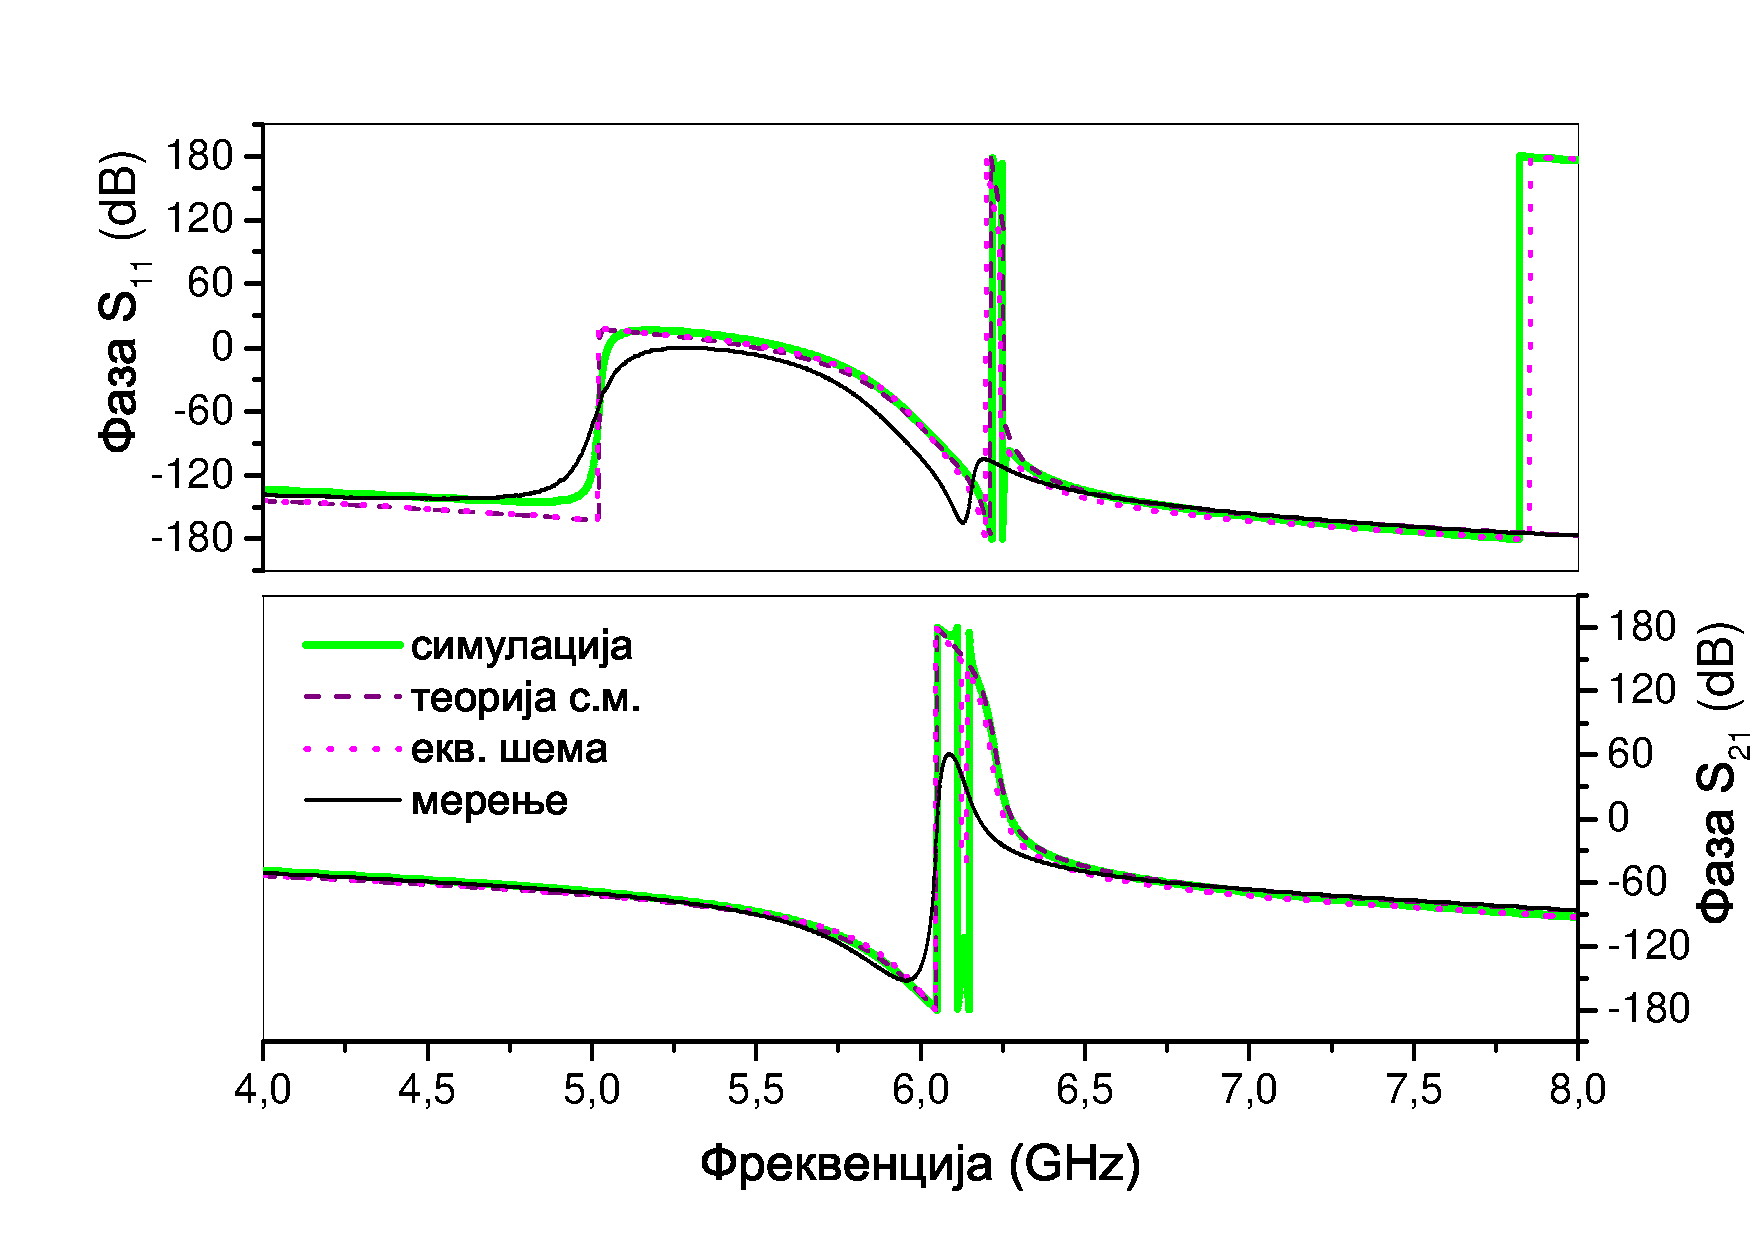
\includegraphics[width=0.8\textwidth]{sl_tsm/pod180/c_faza.pdf}\\
   
   \end{columns} 
\end{frame}
\begin{frame}{}
   \begin{block}{}
    \centering
    \Large\bfseries
       Хвала на пажњи
   \end{block} 
\end{frame}
\end{document}
